\documentclass{beamer}

\mode<presentation>
{
  \usetheme{Luebeck}
  \setbeamercovered{transparent}
}

\usepackage[english]{babel}
\usepackage[latin1]{inputenc}
\usepackage{times}
\usepackage[T1]{fontenc}
\usepackage{graphics}

\title{LSE -- K}

\author{Renaud~Lienhart \and Julien~Quintard}

% If you have a file called "university-logo-filename.xxx", where xxx
% is a graphic format that can be processed by latex or pdflatex,
% resp., then you can add a logo as follows:

% \pgfdeclareimage[height=0.5cm]{university-logo}{university-logo-filename}
% \logo{\pgfuseimage{university-logo}}


% Delete this, if you do not want the table of contents to pop up at
% the beginning of each subsection:
\AtBeginSubsection[]
{
  \begin{frame}<beamer>
    \frametitle{Outline}
    \tableofcontents[currentsection,currentsubsection]
  \end{frame}
}


\begin{document}

\begin{frame}
  \titlepage
\end{frame}

\begin{frame}
  \frametitle{Outline}
  \tableofcontents
\end{frame}


\section{Presentation}

\subsection{Project}

\begin{frame}
  \frametitle{What is K ?}

  \begin{itemize}
  \item
    \texttt{K} is a small kernel (no kidding ?)
  \item
    Delivered in a "tarb-hole"\copyright, similarly to the \texttt{Tiger} project
  \item
    Handles a terminal and keyboard input.
  \item
    Learns you a few basics of the \{x86,IA-32,i686\} Intel architecture.
  \item
    Is monolithic
  \end{itemize}
\end{frame}

\begin{frame}
  \frametitle{What is to be done ?}

  \begin{itemize}
  \item
    Create a multiboot-compatible \texttt{ELF} binary
  \item
    Install a sane execution environment
  \item
    Install our own \texttt{GDT / IDT}
  \item
    Write a terminal and keyboard driver
  \item
    Launch a small shell for human interaction
  \end{itemize}
\end{frame}

\begin{frame}
  \frametitle{What is not to be done ?}

  \begin{itemize}
  \item
    virtual memory
  \item
    some basic privileges handling
  \item
    a multi-task, SMP-aware preemptive operating system (interesting, by the way)
  \item
    IPCs (Inter-Process Communication)
  \item
    a filesystem
  \item
    a graphical user interface
  \end{itemize}
\end{frame}

\begin{frame}
  \frametitle{Sample result}

  \begin{figure}
  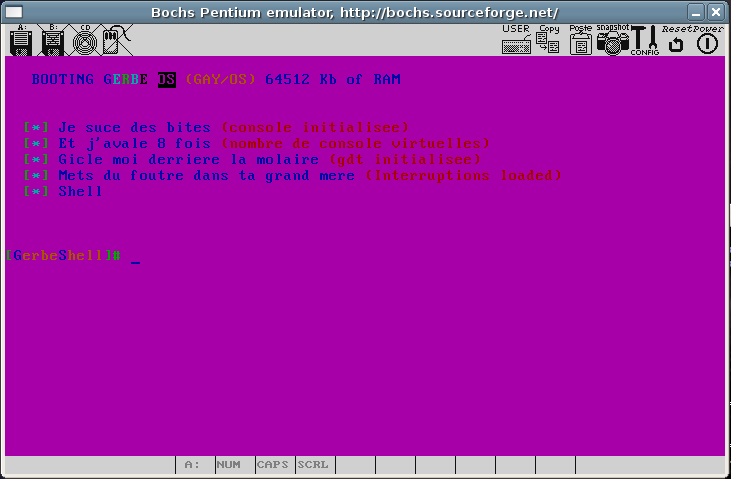
\includegraphics[scale=0.4]{gerbeos.png}
  \end{figure}
\end{frame}


\subsection{Teachers}

\begin{frame}
  \frametitle{Who are we ?}

  \begin{itemize}
  \item
    Renaud Lienhart -- lienha\_r@epita.fr
  \item
    Julien Quintard -- quinta\_j@epita.fr
  \end{itemize}
\end{frame}

\begin{frame}
  \frametitle{Before we start...}

  \begin{itemize}
  \item
    Are you sure you want to discover the hideous internals of the IA-32 architecture ?
  \item
    Debugging a kernel is very hard. Solutions exists. It's not dirty.
  \item
    Don't hesitate to criticize us
  \end{itemize}
  \begin{itemize}
  \item
    Don't be afraid, a kernel is nothing fancy: just an executable binary made with ordinary C code
  \item
    Use the Intel manuals, Luke
  \end{itemize}
\end{frame}

\section{Tools}

\subsection{qemu}

\begin{frame}
  \frametitle{What is it ?}

  \begin{itemize}
  \item
    Virtual machine
  \item
    Easy to use, very fast
  \item
    Embedded real-time shell which gives us machine state
  \item
    Alternatives: Bochs, VMware, a crap second-hand computer
  \end{itemize}
\end{frame}

\begin{frame}
  \frametitle{Screenshot -- Main}

  \begin{figure}
  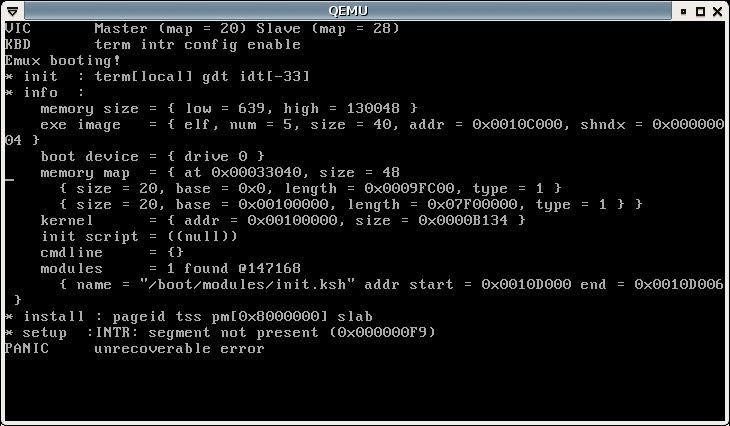
\includegraphics[scale=0.43]{qemu-1.png}
  \end{figure}
\end{frame}

\begin{frame}
  \frametitle{Screenshot -- Shell}

  \begin{figure}
  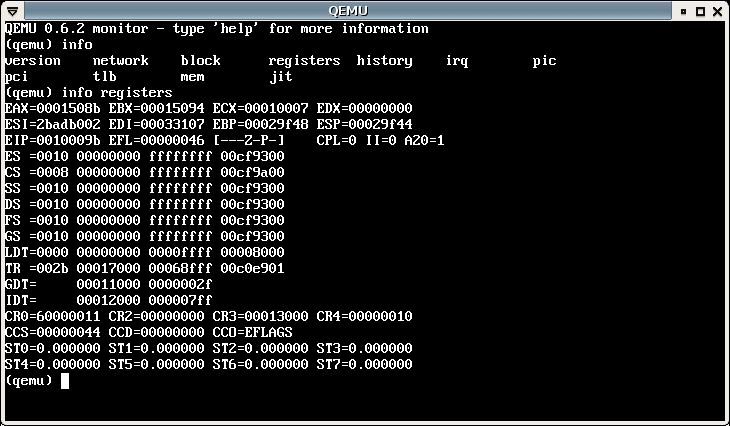
\includegraphics[scale=0.43]{qemu-2.png}
  \end{figure}
\end{frame}

\subsection{gasm, gcc, ld}

\begin{frame}
  \frametitle{Family overview}

  \begin{itemize}
  \item
    GASM: GNU Assembler (.s -> .o)
  \item
    GCC: GNU Compiler Collection (.c -> .o)
  \item
    LD: GNU Linker (.o -> executable)
  \item
    BinUtils: readelf, objdump, ...
  \end{itemize}
\end{frame}

\begin{frame}
  \frametitle{GCC inlined assembly}

  asm (\texttt{assembly template},\\
  \ \ \ \ \ \ \ \ \ : \texttt{output operand} \{, \texttt{output operand}\}*\\
  \ \ \ \ \ \ \ \ \ : \texttt{input operand} \{, \texttt{input operand}\}*\\
  \ \ \ \ \ \ \ \ \ : \texttt{cloberred register} \{, \texttt{clobbered register}\}*\\
  );\\
  \vspace{10pt}
  asm ("mov \%\%cr0, \%\%eax"\\
  \ \ \ \ \ \ \ \ \ "or  \%\%eax, 0x1"\\
  \ \ \ \ \ \ \ \ \ "mov \%\%eax, \%\%cr0"\\
  \ \ \ \ \ \ \ \ \ ::: "\%eax"\\
  );
\end{frame}

\begin{frame}
  \frametitle{GCC arguments}

  \begin{itemize}
  \item
    -nostdinc
  \item
    -nostdlib
  \end{itemize}
  \begin{itemize}
  \item
    gcc -nostdinc -nostdlib windows.c -o kernel32.dll
  \end{itemize}
\end{frame}

\begin{frame}
  \frametitle{LD arguments}

  \begin{itemize}
  \item
    -Ttext <text adress>
  \item
    -e <entry point>
  \end{itemize}
  \begin{itemize}
  \item
    ld -Ttext 0x100000 -e kernel\_kickstart *.o -o mod\_boot
  \end{itemize}
\end{frame}

\subsection{Grub}

\begin{frame}
  \frametitle{What is it ?}

  \begin{itemize}
  \item
    GRUB: Grand Unified Bootloader
  \item
    A mini-OS by itself
  \item
    Collect some informations about the host
  \item
    Switch to 32 bits mode
  \item
    Ask the user which OS to launch
  \item
    Load the specified files in memory and jumps on them
  \end{itemize}
\end{frame}

\begin{frame}
  \frametitle{IBM PC startup}

  \begin{itemize}
  \item<1->
    Loads the BIOS (Basic Input-Output System)
  \item<2->
    Executes the POST (Power-On Self Testing)
  \item<3->
    Scans the boot devices to find a valid boot-sector
  \item<4->
    Once found, jump on it
  \end{itemize}
\end{frame}

\begin{frame}
  \frametitle{menu.lst example}

  timeout 0\\
  default 0\\
\vspace{10pt}
  title  Linux\\
  root   (hd0,0)\\
  kernel /boot/vmlinuz root=/dev/hdc1\\
\vspace{10pt}
  title Kaneton\\
  kernel /mod\_boot\\
  module /mod\_kern\\
  module /mod\_shell
\end{frame}

\section{Memory management}

\subsection{Overview}

\begin{frame}
  \frametitle{What is it ?}

  \begin{itemize}
  \item
    A modern OS needs to restrict tasks's memory accesses
  \item
    Provide an API to give/reclaim memory to processes
  \item
    Is a very complex system nowadays: think of a multi-task OS which handles swapping, mapped files, shared memory and COW pages. All of this blazingly fast and without any security flaw.
  \item
    \$ du -h linux-2.6.11/mm/ ---> 816K
  \end{itemize}
\end{frame}

\begin{frame}
  \frametitle{Address translation mechanism}

  \begin{figure}
  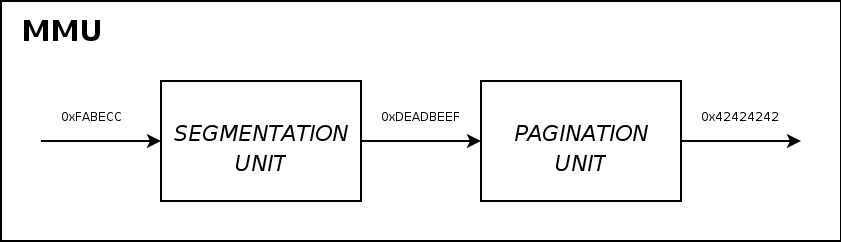
\includegraphics[scale=0.25]{mmu.png}
  \end{figure}
\end{frame}

\subsection{Segmentation}

\begin{frame}
  \frametitle{Definitions}

  \begin{itemize}
  \item
    \texttt{segment}: memory zone, delimited by a starting address ("base") and a size ("limit")
  \item
    \texttt{segment selector}: 16 bits integer which informs us which segment to use
  \item
    \texttt{segment descriptor}: memory structure describing a segment attributes (used only in 32 bits mode)
  \end{itemize}
\end{frame}

\begin{frame}
  \frametitle{Why ?}

  \begin{itemize}
  \item
    The Intel 386 needed a hardware mechanism to isolate concurrent processes
  \item
    This was an easy solution
  \item
    Induces memory fragmentation
  \end{itemize}
\end{frame}

\begin{frame}
  \frametitle{Real mode -- schema}

  \begin{figure}
  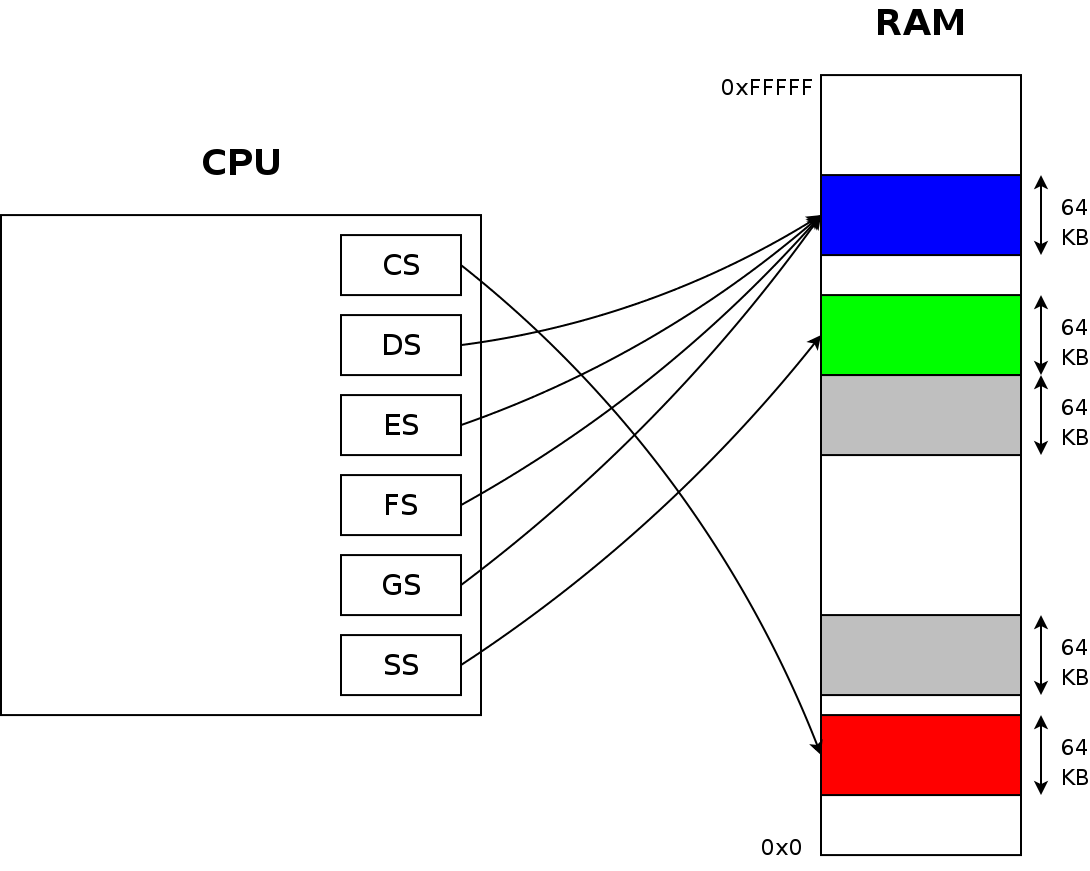
\includegraphics[scale=0.16]{real.png}
  \end{figure}
\end{frame}

\begin{frame}
  \frametitle{Real mode -- translation}

  addr20\_t translate\_real(short segment, addr16\_t addr)\\
 \{\\
  \ \ \ \ if (!is\_defined(segment))\\
  \ \ \ \ \ \ \ \ segment = content\_of(\texttt{segment\_register});\\
  \ \ \ \ return (segment << 4) + addr;\\
 \}\\

  \vspace{10pt}

  0xABCD:0x4242 ---> (0xABCD << 4) + 0x4242 ---> 0x2F176
\end{frame}

\begin{frame}
  \frametitle{Real mode -- limitations}

  \begin{itemize}
  \item
    Could not address more than $2^{20}$ == 1 MB of memory
  \item
    Each process could only address $2^{16}$ == 64 KB of memory at a time
  \item
    Each segment has a fixed length
  \end{itemize}
\end{frame}

\begin{frame}
  \frametitle{Protected mode -- schema}

  \begin{figure}
  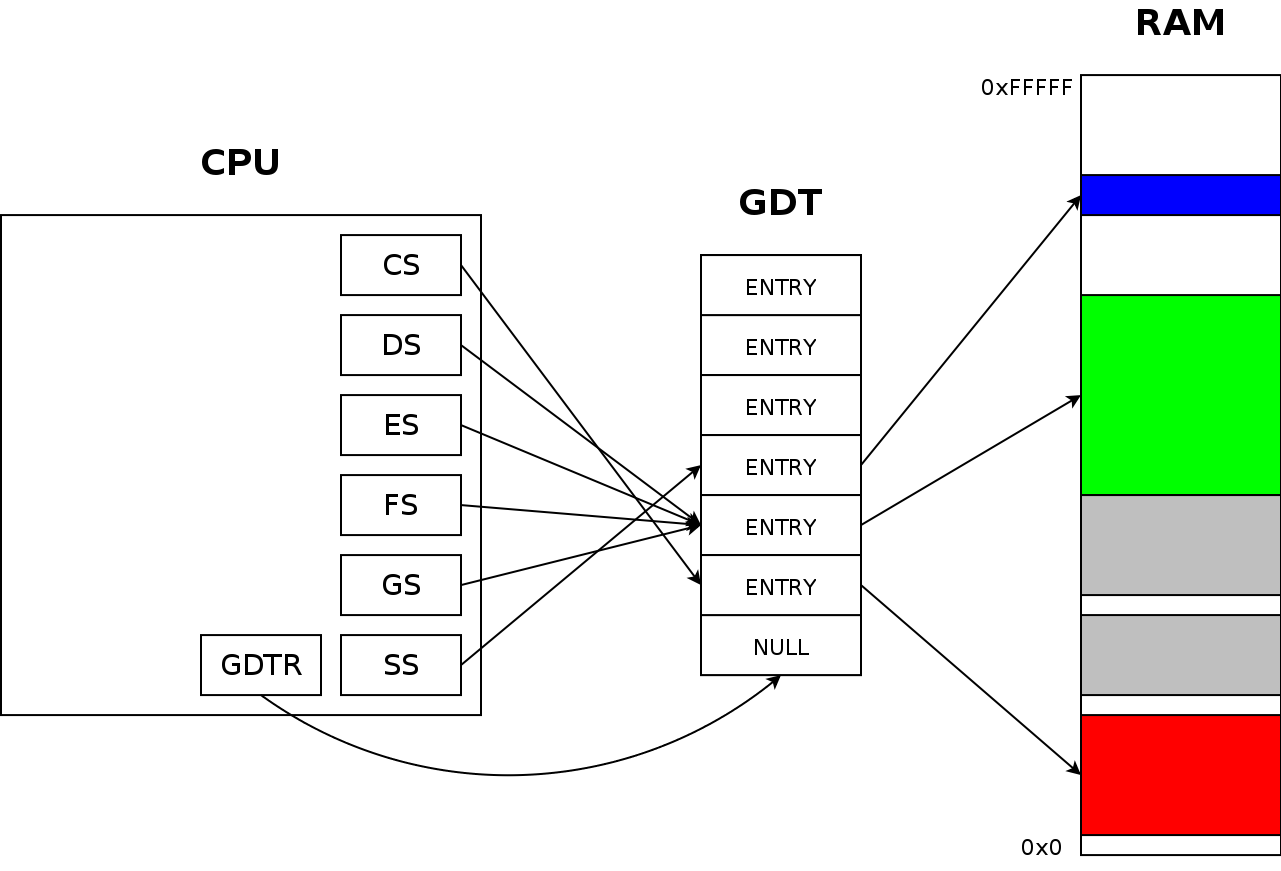
\includegraphics[scale=0.15]{prot.png}
  \end{figure}
\end{frame}

\begin{frame}
  \frametitle{Protected mode -- translation}

  addr32\_t translate\_prot(addr32\_t addr)\\
 \{\\
  \ \ \ \ segment\_sel = content\_of(\texttt{segment\_register});\\
  \ \ \ \ seg\_base = gdt[segment\_sel].base;\\
  \ \ \ \ seg\_limit = gdt[segment\_sel].limit;\\
  \ \ \ \ seg\_prot = gdt[segment\_sel].prot;\\
  \ \ \ \ if (addr > seg\_limit)\\
  \ \ \ \ \ \ \ \ /* exception */;\\
  \ \ \ \ if (!is\_compatible(access\_type(\texttt{current\_operation}), seg\_prot))\\
  \ \ \ \ \ \ \ \ /* exception */;\\
  \ \ \ \ return seg\_base + addr;\\
 \}
\end{frame}

\begin{frame}
  \frametitle{Protected mode -- limitations}

  \begin{itemize}
  \item<1->
    Manipulation is painful
  \item<1->
    Obsoleted by pagination -- we could get rid of it but compatibility-descendance is required
  \end{itemize}
  \begin{itemize}
  \item<2->
    In order not to care about it, we just have to create a "flat" segmentation model
  \item<2->
    2 kernel segments and 2 user segments which starts at 0x0 and covers 4GB of memory
  \item<2->
    Creepy, isn't it ?
  \end{itemize}
\end{frame}

\begin{frame}
  \frametitle{GDT -- gdtr}

  \begin{figure}
  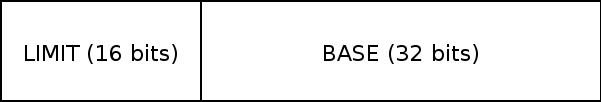
\includegraphics[scale=0.3]{gdtr.png}
  \end{figure}
  We can't encode 48 bits in an instruction, so we have to fill a structure in memory and give the processor a pointer to it:\\
  \vspace{10pt}
  gdtr.limit = 42;\\
  gdtr.base = 0x1000;\\
  asm ("lgdt (\%0)", :: "m" (gdtr));
\end{frame}

\begin{frame}
  \frametitle{GDT -- entry}

  \begin{figure}
  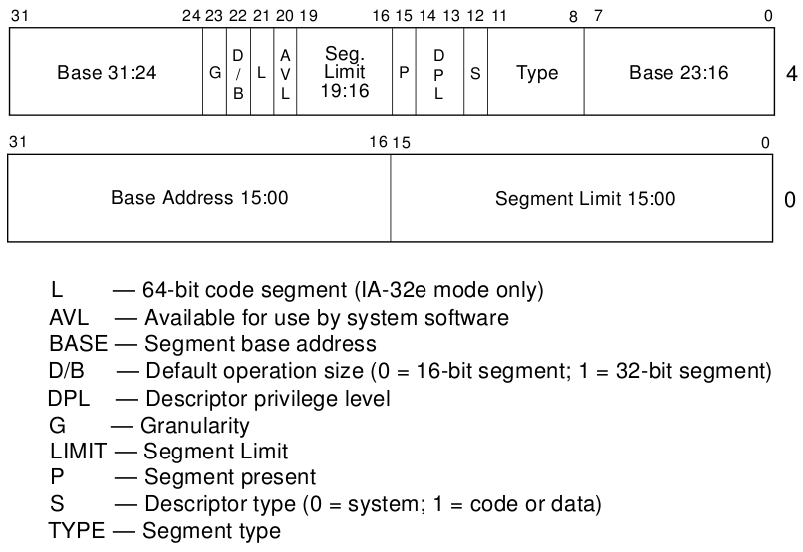
\includegraphics[scale=0.35]{gdte.png}
  \end{figure}
\end{frame}

\begin{frame}
  \frametitle{GDT -- registers}

  \begin{itemize}
  \item
    CS: Code Segment (\texttt{jmp}, ...)
  \item
    DS, ES, FS, GS: Data Segment (\texttt{mov}, ...)
  \item
    SS: Stack Segment (\texttt{push}, ...)
  \end{itemize}
  \begin{figure}
  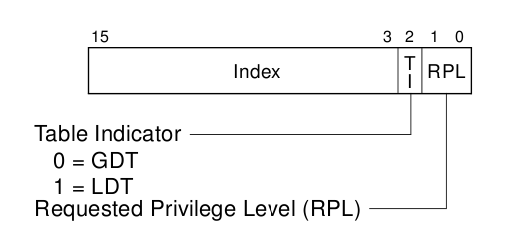
\includegraphics[scale=0.5]{segreg.png}
  \end{figure}
\end{frame}

\subsection{Pagination}

\begin{frame}
  \frametitle{Requirements}

  \begin{itemize}
  \item
    Fragmentation should not be an issue as RAM is UMA: we don't care about contiguous memory.
  \item
    Need a way to efficiently share memory
  \end{itemize}
\end{frame}

\begin{frame}
  \frametitle{Definitions}

  \begin{itemize}
  \item
    RAM is logically divised in chunks called \texttt{pages} (4096 Bytes on x86)
  \item
    A \texttt{page} refers to an adress range in a process virtual address space.
  \item
    A \texttt{page frame} refers to an address range in physical memory.
  \item
    Therefore, we say that a page is \texttt{mapped} on a page frame.
  \end{itemize}
\end{frame}

\begin{frame}
  \frametitle{Translation}

  We need a way to bind virtual addresses to their physical equivalents:\\
  What about a simple map ?

  \begin{figure}
  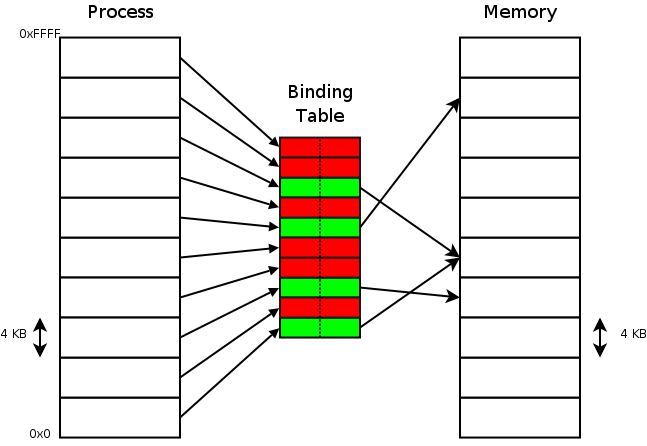
\includegraphics[scale=0.25]{bind.png}
  \end{figure}
\end{frame}

\begin{frame}
  \frametitle{Valability}

  A quick computation: $\frac{2^{32}}{4096} * 8 = 8388608$\\
  We need 8 MB to describe a 4 GB address space!\\
  Therefore a simple binding map is not a viable solution.\\
  \vspace{10pt}
  A reasonable solution to describe an address space is to use a N-Tree. The nodes of this tree are often called \texttt{page tables}.
\end{frame}

\begin{frame}
  \frametitle{Page tables}

  \begin{figure}
  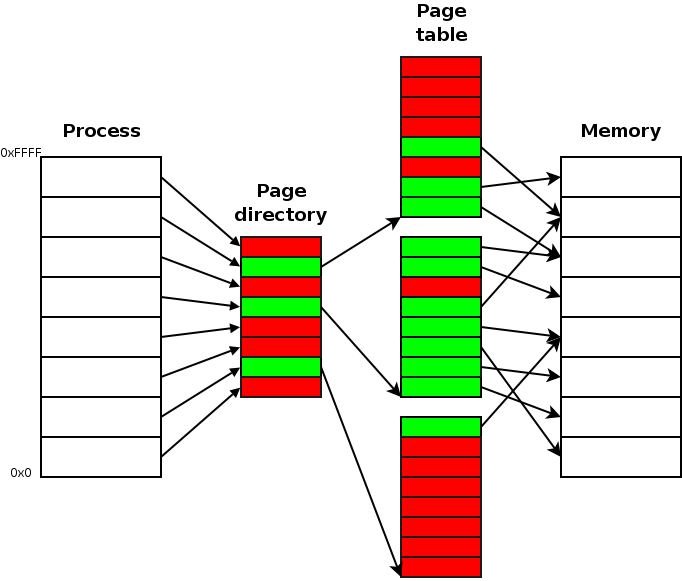
\includegraphics[scale=0.25]{pagetable.png}
  \end{figure}
\end{frame}

\begin{frame}
  \frametitle{Translation mechanism}

  \begin{figure}
  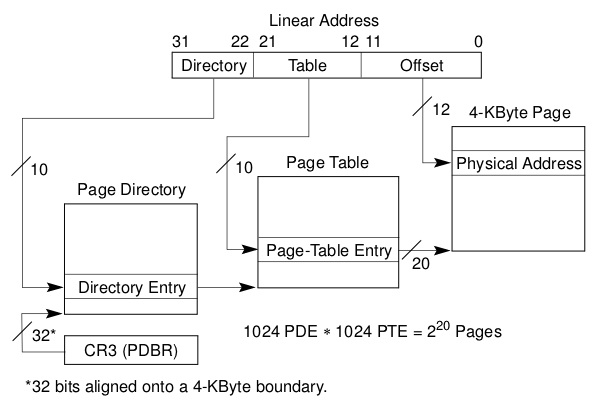
\includegraphics[scale=0.5]{virt.png}
  \end{figure}
\end{frame}

\begin{frame}
  \frametitle{PDE}

  \begin{figure}
  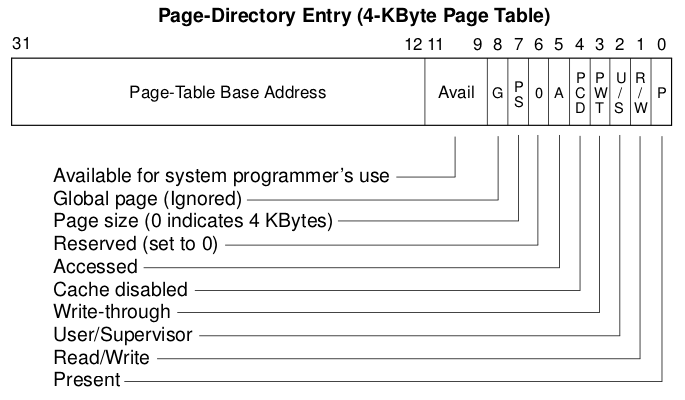
\includegraphics[scale=0.4]{pde.png}
  \end{figure}
\end{frame}

\begin{frame}
  \frametitle{PTE}

  \begin{figure}
  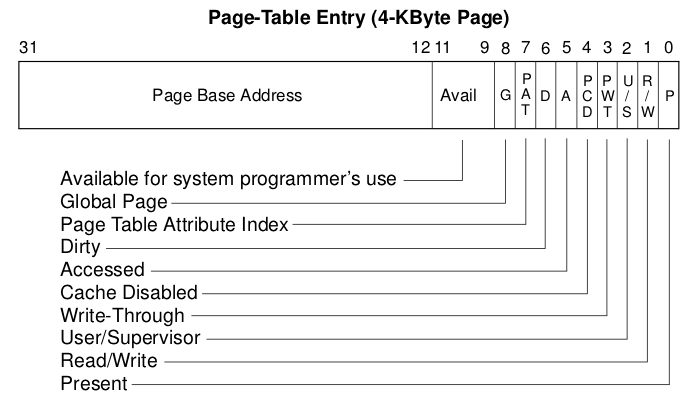
\includegraphics[scale=0.4]{pte.png}
  \end{figure}
\end{frame}

\begin{frame}
  \frametitle{TLB}

  Translating a virtual address costs 2 memory accesses.\\
  \vspace{10pt}
  The \texttt{Translation Lookaside Buffer} is an on-core cache of recently used translations.\\
  It is the responsibility of the system programmer to maintain its consistency (eurk).
  \vspace{10pt}
  \begin{itemize}
  \item
    Invalidate one entry: \texttt{invlpg}
  \item
    Invalidate the whole TLB: overwrite \texttt{cr3}
  \end{itemize}
\end{frame}

\section{Interrupts}

\subsection{Generalities}

\begin{frame}
  \frametitle{Peripherals communication}

  The devices have two mechanisms in order to communicate with the CPU:\\
  \begin{itemize}
  \item
    Polling
  \item
    Interrupts
  \end{itemize}
\end{frame}

\begin{frame}
  \frametitle{Polling}

  The CPU constantly polls the device internal \texttt{status register}. When the device has something to transmit, it sets its \texttt{status register} to a defined value and waits for the CPU to acknowledge the transfer.\\
  \begin{itemize}
  \item
    Easy to conceive, but wastes too much system ressources
  \item
    Latency is non-deterministic and frequently bad: when you're moving the mice, you expect the pointer to move immediatly
  \item
    Nonetheless subsystems like USB controllers uses polling (1000 HZ) and raises a single interrupt to prevent the CPU
  \end{itemize}
\end{frame}

\begin{frame}
  \frametitle{Interrupts -- mechanism}

  When a device wants to communicate with the CPU, it raises an \texttt{interrupt}. The CPU preempts the current running process in order to execute the \texttt{interrupt handler} (also called \texttt{Interrupt Service Routine} (ISR)) associated with the \texttt{IRQ line}.\\
\end{frame}

\begin{frame}
  \frametitle{Interrupts -- example}

  \begin{itemize}
  \item<1->
    The printer raises an interrupt on IRQ 42.
  \item<2->
    The CPU preempts the current job and launches the interrupt handler associated with IRQ 42. Normally the printer device driver registered this IRQ and associated its handler to it.
  \item<3->
    The printer driver asks "WTF ?" to the printer which responds that there is no more paper.
  \item<4->
    A decision is made (in this case, transmit a message to userland to avert the printer needs paper).
  \item<5->
    The treatment is completed, the CPU resumes the preempted job.
  \end{itemize}
\end{frame}

\begin{frame}
  \frametitle{Interrupts -- problems}

  \begin{itemize}
  \item
    Race conditions everywhere: interrupts are asynchronous, so proper locking policy must be ensured
  \item
    The IRQ handler must be as fast as possible: they can preempt real-time tasks.
  \item
    High interrupt rate can cause the system to collapse. Imagine a network card receiving a packet every ms and taking 2ms to process it.
  \end{itemize}
\end{frame}

\begin{frame}
  \frametitle{Interrupts -- schema}

  \begin{figure}
  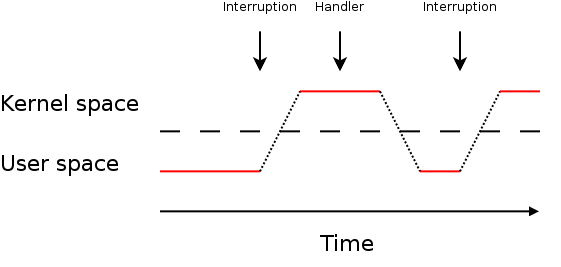
\includegraphics[scale=0.38]{interrupts.png}
  \end{figure}
\end{frame}

\subsection{IDT}

\begin{frame}
  \frametitle{IDT -- overview}

  \begin{figure}
  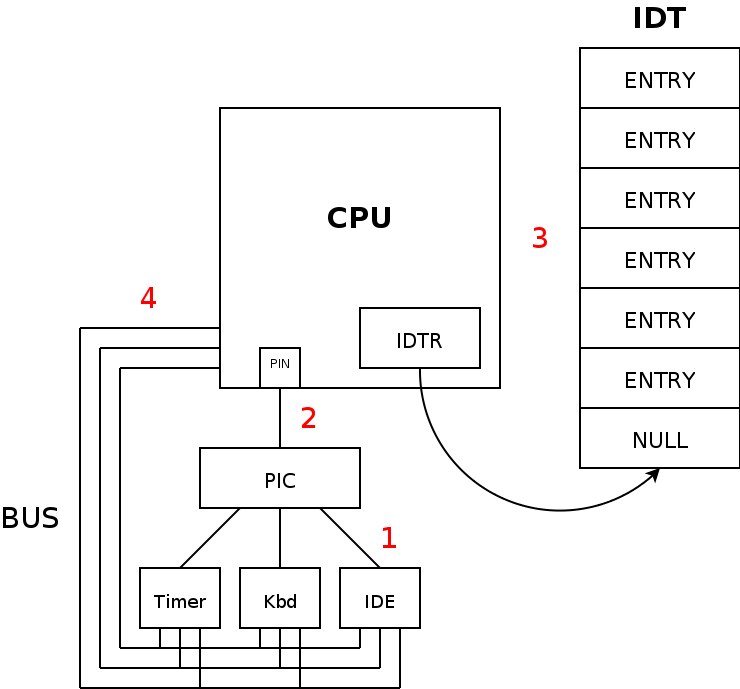
\includegraphics[scale=0.2]{idtoverview.png}
  \end{figure}
\end{frame}

\begin{frame}
  \frametitle{IDT -- idtr}

  \begin{figure}
  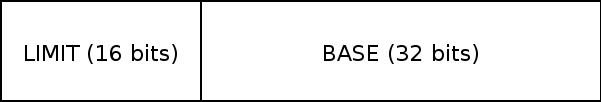
\includegraphics[scale=0.3]{idtr.png}
  \end{figure}
  We can't encode 48 bits in an instruction, so we have to fill a structure in memory and give the processor a pointer to it:\\
  \vspace{10pt}
  idtr.limit = 42;\\
  idtr.base = 0x1000;\\
  asm ("lidt (\%0)", :: "m" (idtr));
\end{frame}

\begin{frame}
  \frametitle{IDT -- entry}

  \begin{figure}
  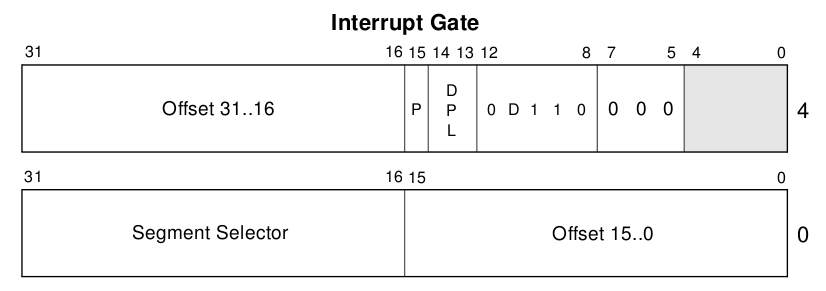
\includegraphics[scale=0.38]{idte.png}
  \end{figure}
\end{frame}

\subsection{PIC}

\begin{frame}
  \frametitle{What is it ?}

  \begin{itemize}
  \item
    The PIC (Programmable Interrupt Controller) is an electronic circuit (8259) external to the CPU
  \item
    Acts as a multiplexer in order to keep the processor having a pin for each IRQ line
  \item
    Is outdated, nowadays on-core APIC (add "Advanced") is quietly replacing it
  \end{itemize}
\end{frame}

\begin{frame}
  \frametitle{Defaults}

    The PIC handles only 15 IRQs lines and several of them are already reserved for legacy devices like the timer or the keyboard.\\
    Actually only 5 IRQs are really usable. Therefore the operating system is often forced to make devices share an IRQ line. This leads to a performance penalty (the OS must scan each device on the IRQ to know which one raised the interrupt) and stability issues (for Windows).\\
  Furthermore, PIC manipulation is simply a PITA.
\end{frame}

\begin{frame}
  \frametitle{Schema}

  \begin{figure}
  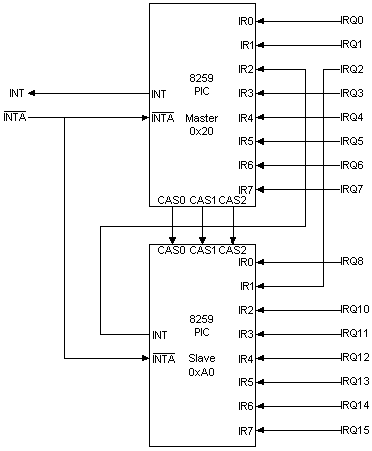
\includegraphics[scale=0.42]{pic.png}
  \end{figure}
\end{frame}

\begin{frame}
  \frametitle{I/O ports}

  In order to communicate with external devices, Intel created the holy I/O ports.\\
  An I/O port is a communication channel to legacy devices. They are static (we can't bind them dynamically), slow and deprecated by I/O memory mapping.\\
  \vspace{20pt}
  /* send \%al to IO/port number \%dx */\\
  out \%al, \%dx;\\
  /* get \%al from IO/port number \%dx */\\
  in \%dx, \%ax;
\end{frame}

\section{Drivers}

\subsection{Console}

\begin{frame}
  \frametitle{VGA memory}

  \begin{itemize}
  \item
    Located at 0xB8000 and is composed of 80x25 characters
  \item
    Each character on the screen is made of 16 bits:
    \begin{itemize}
    \item
      1 byte for the character itself
    \item
      1 byte for its attributes (color, ...)
    \end{itemize}
  \end{itemize}
  \begin{figure}
  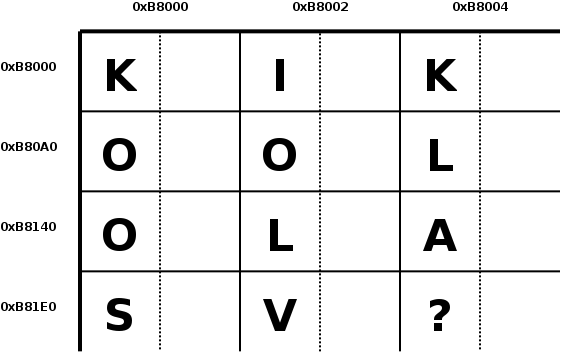
\includegraphics[scale=0.25]{vga.png}
  \end{figure}
\end{frame}

\subsection{Keyboard}

\begin{frame}
  \frametitle{How it works}

  The keyboard, when receiving an event (pressing or releasing a key), raises an interrupt on IRQ1.\\
  Then, using IO/ports, we just have to read the keyboard internal buffer.
\end{frame}

\end{document}
